\documentclass[]{article}

\usepackage{sectsty}

\usepackage[parfill]{parskip}

\usepackage{hyperref}

\usepackage[T1]{fontenc}

\usepackage{graphicx}

\usepackage[T1]{fontenc}

\sectionfont{\fontsize{10}{10}\selectfont}


\begin{document}


\author{
  Nikhil Chaturvedi\\
  \texttt{2013CS50291}
  \and
  Harman Kumar\\
  \texttt{2013CS10224}
}

\title{Game Of Thrones Wiki}
\maketitle



\section{Overall Design}

\begin{flushleft}

We present a complete database for the most popular TV series, Game of Thrones. We have over 1000 character stats and prediction about their survival based on popularity, number of dead relatives they have and how good their house is doing.

The system allows users to create password secured accounts in order in order to access the GOT Wiki. We also have a separate admin login which allows us to add new information to our databases using a form.\\

You can find the ER diagram of the project at the end of the document.

\end{flushleft} 

\vspace{25px}

\section{Data Source}

We took our data from three sources:

\begin{itemize}
\item A collection of all battles in game of thrones at\\ 
https://github.com/chrisalbon/war\_of\_the\_five\_kings\_dataset


\item Information about characters, when they died and a brief boi about the characters.\\
http://allendowney.blogspot.in/2015/03/bayesian-survival-analysis-for-game-of.html


\item A collection of all the character predictions. This dataset contains an expanded view on character deaths, including predictions of how likely they are to die. (Prediction's come from A Song of Ice and Data's algorithm)\\
https://got.show/

Following is the schema of the data

\begin{figure}
\centering
        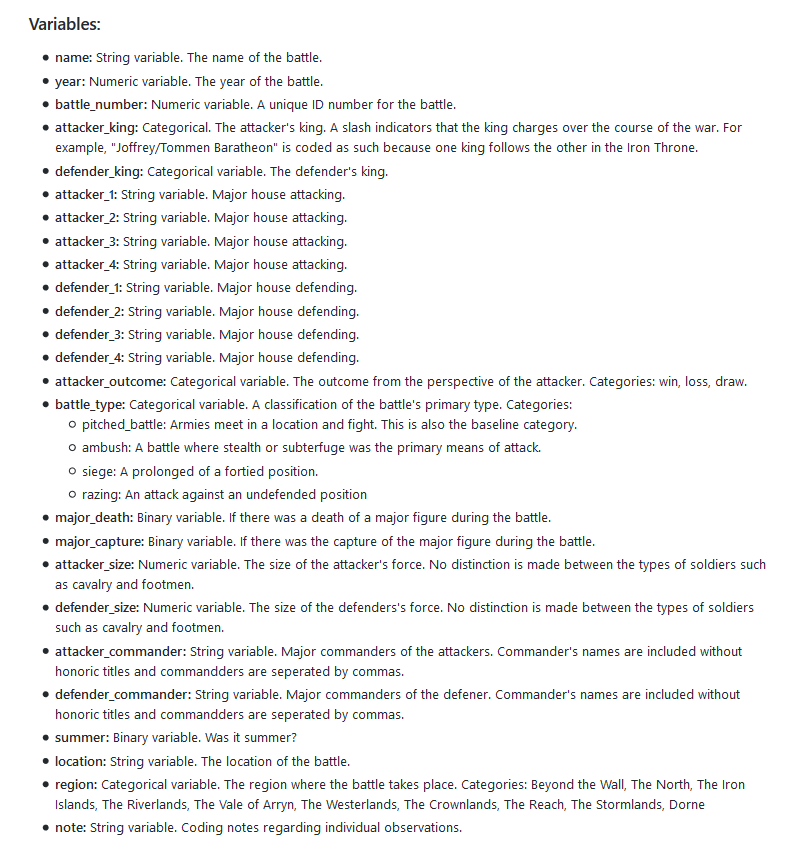
\includegraphics[totalheight=16cm]{battles.png}
        \caption{Schema of the battles dataset}
\end{figure}


\begin{figure}
\centering
        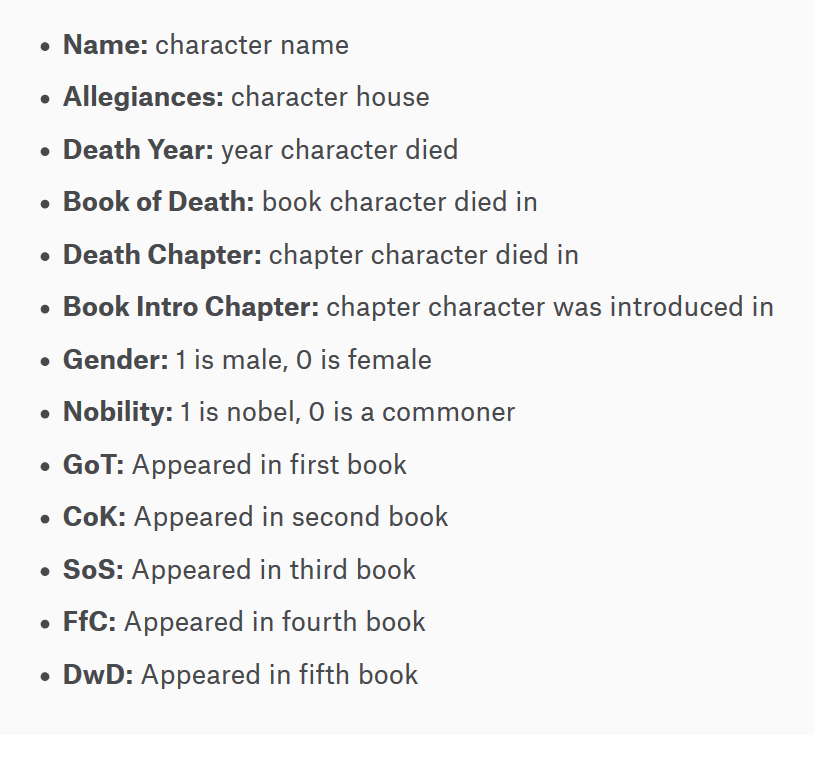
\includegraphics[totalheight=10cm]{deaths.png}
        \caption{Schema of the character deaths dataset}
\end{figure}


\begin{figure}
\centering
        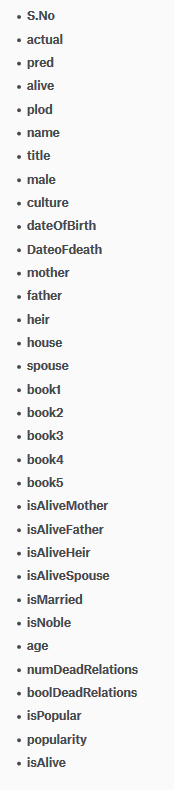
\includegraphics[totalheight=13cm]{prediction.png}
		\caption{Schema of the prediction Dataset}
\end{figure}


\end{itemize}

\vspace{25px}

A python script was written to cleanup the data, create the database, specify the schema of tables, various constraints, triggers, do indexing on the data, create virtual and materialized views and load the data into the tables. 


\section{Functionality and Components}

\begin{itemize}
\item \textbf{View Interesting Characters:}\\
Our dataset has a field that species whether a character is interesting or not. Using this the give the user an option to filter out the main characters.

\item \textbf{Find a character:}\\
In our frontend we have the search bar functionality using which we can search for a house or a character. This is a much required functionality as there are over 1000 characters in GOT.

\item \textbf{View Interesting Characters:}\\
Our dataset has a field that species wheteher a character is interesting or not. Using this the give the user an option to filter out the main characters.

\item \textbf{Sort by Most Likely to Die:}\\
Our predictions dataset has a field that predicts the likelihood of a character dying. In order to view spoilers, one can sort the characters by this field and find out which characters would die next.

\item \textbf{Sort By Popularity:}\\
Sort characters by popularity to see the main charcters and then the side characters. 



\end{itemize}

\end{document}